\documentclass[a4paper, 12pt]{article}
\usepackage[total={17cm,25cm}, top=2.5cm, left=2.5cm, right=2.5cm,  includefoot]{geometry}
\usepackage[utf8]{inputenc}
\usepackage{array}
\usepackage{multirow}
\usepackage{hhline}
\usepackage{gensymb}
\usepackage{graphicx}
\graphicspath{ {} }
\usepackage[czech]{babel}
\usepackage{enumitem}
\usepackage{pdfpages}
\usepackage{amsmath}
\usepackage{verbatim}
\usepackage{listings}
\usepackage{hyperref}
\usepackage{amssymb}


\pagestyle{empty} % vypne číslování stránek




\usepackage[OT2,OT1]{fontenc}
\newcommand\cyr
{
\renewcommand\rmdefault{wncyr}
\renewcommand\sfdefault{wncyss}
\renewcommand\encodingdefault{OT2}
\normalfont
\selectfont
}
\DeclareTextFontCommand{\textcyr}{\cyr}
\def\cprime{\char"7E }
\def\cdprime{\char"7F }
\def\eoborotnoye{\char’013}
\def\Eoborotnoye{\char’003}


\begin{document}



\begin{titlepage}
\begin{center}
\noindent
\Large \textbf{České vysoké učení technické v Praze }\\ Fakulta stavební
\vspace{5cm}

\huge

%vložení loga cvut
\begin{figure}[h!]
	\centering
	
\includegraphics[width=7cm]{logo.png}
\end{figure}

\vspace{0.5cm}

Úvod do zpracování prostorových dat \\

\vspace{3cm}

\Huge  
Přírodní prvky okresu Strakonice\\

\vspace{2cm}

\Large
Bc. Michal Janovský \\
Bc. Petra Pasovská \\

\end{center}

\end{titlepage}




\pagestyle{plain}     % zapne obyčejné číslování
\setcounter{page}{1}  % nastaví čítač stránek znovu od jedné

\tableofcontents
\newpage


\section{Úvod}
Tato dokumentace je součástí semestrálního projektu v předmětu Úvod do zpracování prostorových dat pod vedením Ing. Martina Landy, Ph. D. Hlavním cílem projektu bylo vytvoření databáze, nad níž budou následně volány prostorové dotazy.\\
\\
Autoři si sami zvolili takové téma, které je zajímá a sami si vyhledávali zdroje. Jedním z hlavních cílů tohoto projektu je mimojiné prozkoumání jednotlivých zdrojů. Za tímto účelem bylo pro analýzu vybráno menší zájmové území - okres Strakonice (nebo Jihočeskký kraj??). \\
\\
Přírodní prvky byly zvoleny z toho důvodu, neboť autoři mají velmi kladný vztah k přírodě. Navíc v rámci přírodních prvků je prováděno velké množství analýz, díky čemuž je pro toto téma mnoho dat a je zde větší množství zdrojů, které mohou autoři prozkoumat.\\
\\
Výsledkem práce je databáze obsahující několik bodových, liniových a polygonových vrstev.

\clearpage
\section{Zdroje dat}
Pro tento projekt bylo použito několik zdrojů veřejně dostupných zdrojů.

\subsection{DIBAVOD}
Digitální báze vodohospodářských dat, zkráceně DIBAVOD, je referenční geografická databáze, která je součástí nadstavby ZABAGED (Základní báze geografických dat ČR - digitální topografický model území ČR odvozený z mapového obrazu Základní mapy České republiky 1:10 000). Primárně byla vytvořena pro tvorbu tématických kartografických výstupů s vodohospodářskou tematikou a tematikou ochrany vod. \\
\\
Obecně lze DIBAVOD považovat jako databázi podkladových dat pro kategorii vodstvo pro ZABAGED. Uživatel má možnost si zdarma stáhnout data ve formátu shapefile v několika podkategoriích, např. chráněná území, objekty na toku, záplavová území či měřící a kontrolní mmísta povrchových vod. 

\begin{figure}[h!]
	\centering
	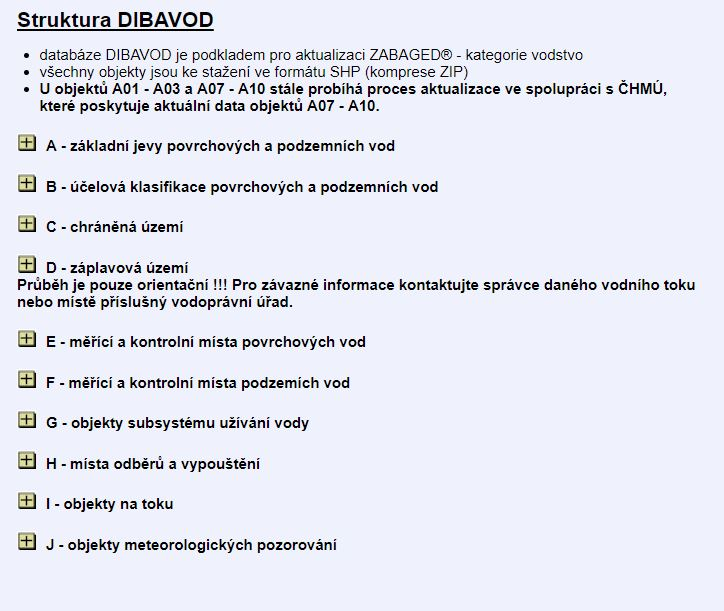
\includegraphics[width=13cm]{pictures/dibavod.jpg}
	\caption{Struktura dat DIBAVOD}
\end{figure}

\subsection{OpenStreetMap}
OpenStreetMap je projekt, jehož cílem je tvorba volně dostupných geografických dat a následně jejich vizualizace do podoby silniční mapy, uliční mapy měst atd. Tato vektorová data jsou poskytována pod licencí Open Database Licence. \\
\\
Jedná se o taková zdrojová data, která může kdokoliv upravit. Díky tomu se na tvorbě může podílet v podstatě kdokoliv, v současné době navíc existují i pluginy, které umožňnují stáhnutí OMS do Garminu či smartphonů. 

\begin{figure}[h!]
	\centering
	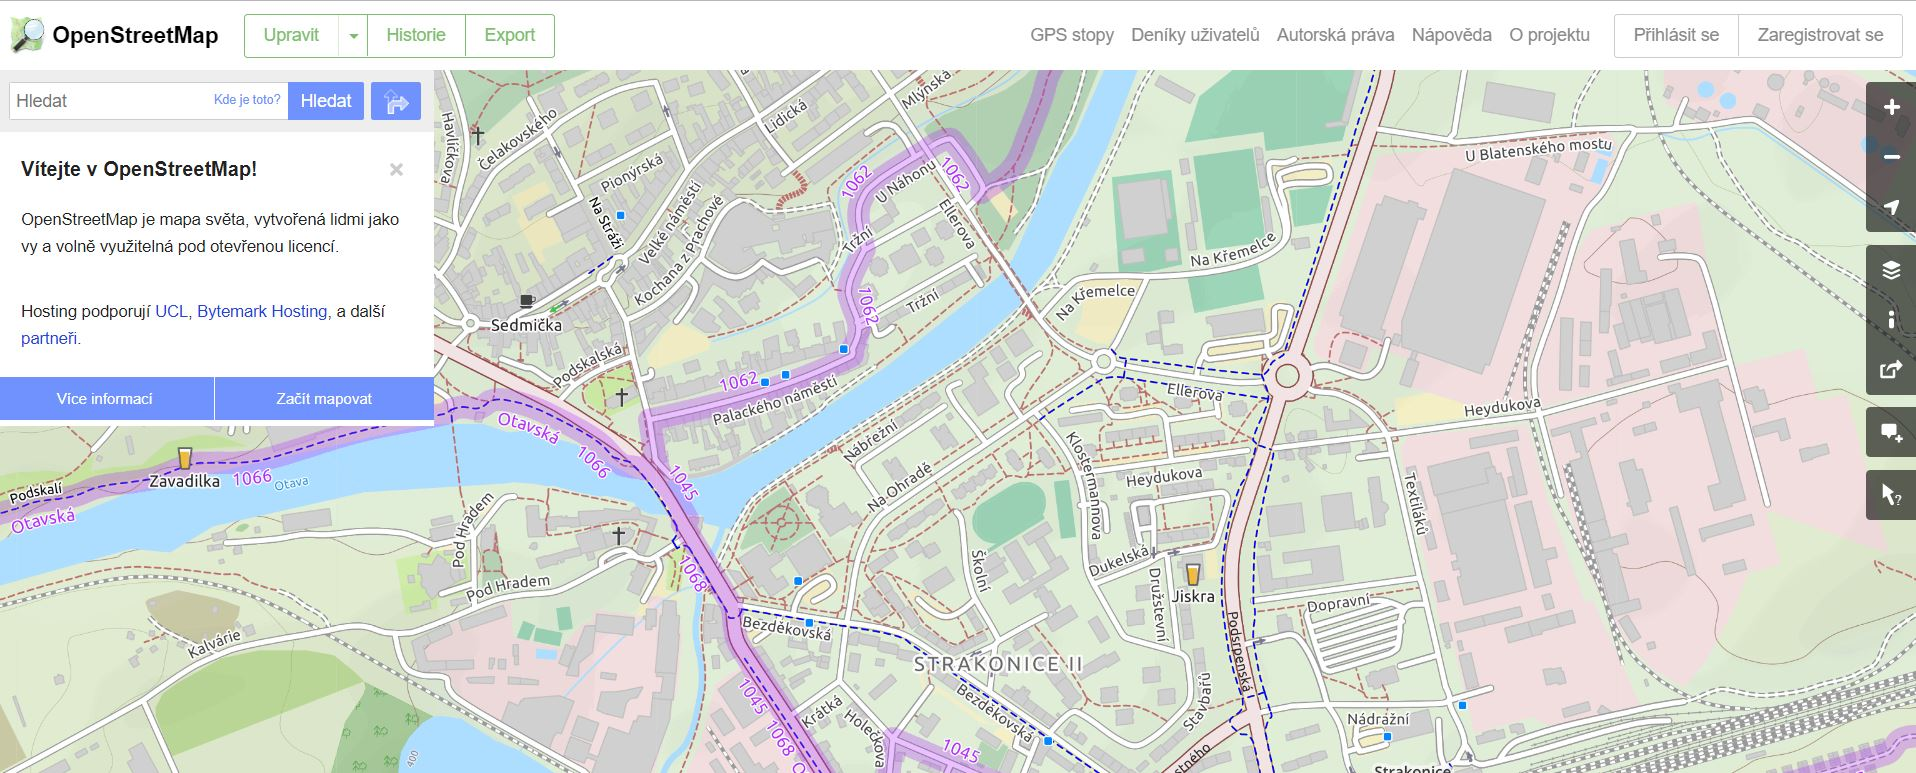
\includegraphics[width=14cm]{pictures/osm.jpg}
	\caption{Ukázka OpenStreetMap pro část Strakonic}
\end{figure}


\subsection{ArcČR 500}
ArcČR 500 je digitální vektorová geografická databáze České republiky. Data vznikla ve spolupráci ARCDATA Praha, s.r.o., Zeměměřického úřadu a Českého statistického úřadu. Data jsou pro uživatele k dispozici zdarma. \\
\\
Data lze rozdělit do tří hlavních složek - Administrativní členění, Geografické prvky a Klady a sítě. Pro projekt byly zahrnuty jen určité vrstvy z kategorie Geografické prvky. 

\begin{figure}[h!]
	\centering
	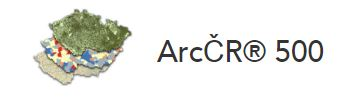
\includegraphics[width=8cm]{pictures/arccr.jpg}
	\caption{Logo ArcČR 500}
\end{figure}

\subsection{AOPK ČR}
Agentura Ochrany Přírody a Krajiny ČR nabízí datové sady týkající se národně i mezinárodně chráněných územích či druzích, památných stromech, biotopech, rezervacích, geoparcích či mokřadech. Data jsou v souřadnicovém systému WGS84 a organizace nabízí řadu formátů, ve kterých lze data stáhnout.\\
\\
Agentura spadá pod Ministerstvo životního prostředí a v roce 2017 získala ocenění na evropské konferenci INSPIRE ve Štrasburku. 
\clearpage
\begin{figure}[h!]
	\centering
	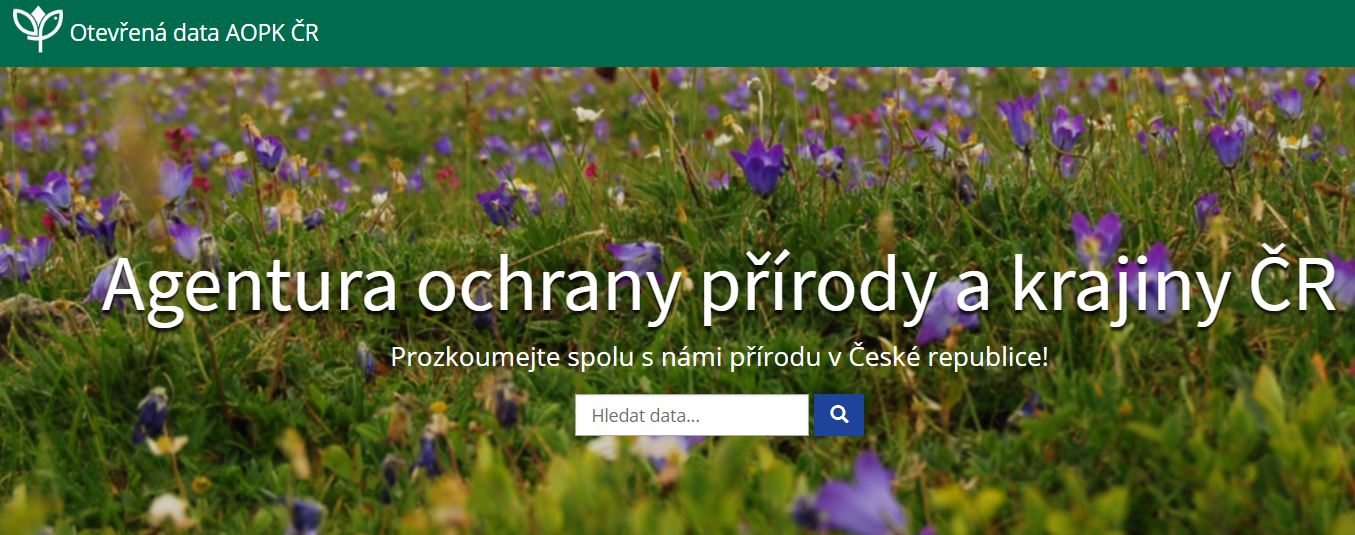
\includegraphics[width=12cm]{pictures/aopk.jpg}
	\caption{Agentura ochrany přírody a krajiny ČR}
\end{figure}


\subsection{ČSÚ}
Český statistický úřad je ústřední orgán státní správy České republiky. Je nezávislý na vládě a politických stranách. ČSÚ zajišťuje zpracování a zveřejňování údajů, sestavuje souhrnné statistické charakteristiky vývoje národního hospodářství, zpracovává analýzy, zároveň shromažďuje i zahraniční statistické informace a jednou za 10 let provádí Sčítání lidu. \\
\\
Všechna data a informace jsou na serveru zdarma pro státní správu i běžného užiivatele. Data jsou většinou k dispozici ve dvou formátech - ve formátu XML a CVS. Jedním ze známých produktů ČSÚ jsou také výsledky voleb.

\begin{figure}[h!]
	\centering
	
\includegraphics[width=12cm]{pictures/csu.jpg}
	\caption{Logo Českého statistického úřadu}
\end{figure}


\section{Software}
\subsection{QGIS}
Tvorba databáze a prostorových dotazů probíhala ve frameworku QGIS. Aplikace QGIS je velmi podobná programu ArcGIS od společnosti ESRI, velkou výhodou však je to, že se jedná o multiplatformní program, který je zcela zdarma. V dnešní době je velmi rozšířen a existuje mnoho zásuvných modulů (pluginů), které mají v sobě naimplementovány často používané funkce.\\
\\

\begin{figure}[h!]
	\centering
	
\includegraphics[width=5cm]{pictures/qgis.png}
	\caption{QGIS}
\end{figure}

Ve frameworku QGIS má uživatel možnost vytvářet, editovat či čistě jen prohlížet rastrová a vektorová geodata. V rámci programu je možné provádět prostorové a atributové dotazy. Zároveň je možná práce s webovými službami OGC. Zároveň může uživatel importovat data s oddělenými hodnotami (př. CSV) či připojit tabulková data.\\
\\

\begin{figure}[h!]
	\centering
	
\includegraphics[width=8cm]{pictures/qgis.jpg}
	\caption{QGIS}
\end{figure}

\subsection{PostGIS}
PostGIS je open source program, který je nadstavbou objektově relačního databázového systému PostgreSQL, jenž rozšiřuje podporu systému o geograficky objekty. PostGIS podporuje mimo QGIS např. Mapnik nebo Quantum GIS. Tato nadstavba umožňuje manipulovat a analyzovat geodata za pomoci dotazovacího jazyka SQL. 

\begin{figure}[h!]
	\centering
	
\includegraphics[width=10cm]{pictures/postgis.png}
	\caption{PostGIS}
\end{figure}


\section{Praktická část}
\subsection{Databáze}
Nejprve bylo nutné se připojit na server, na němž bude uložena vytvořená geodatabáze. Připojení může probíhat prostřednictvím příkazové řádky nebo přes konzoli v prostředí QGIS. Databáze pro tento projekt byla vytvářena přes konzoli. Připojení pomocí příkazové řádky bylo několikrát vyzkoušeno v rámci cvíčení, navíc lze na internetu najít spoustu návodů. Přesto nemají autoři takové množství zkušeností, aby si věřili natolik, že přes příkazovou řádku nahrají vše bez chyb. 

\begin{figure}[h!]
	\centering
	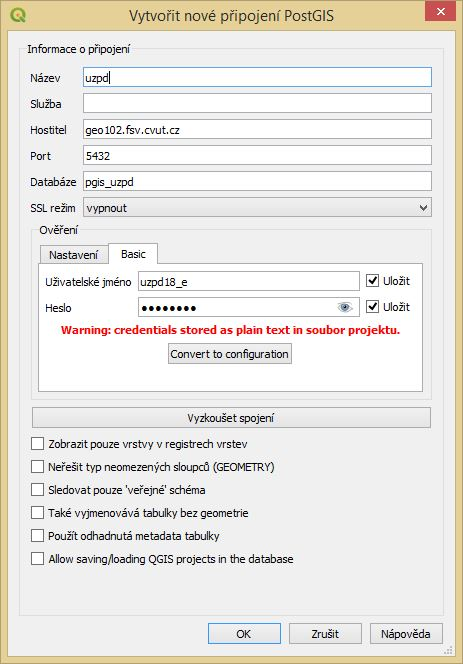
\includegraphics[width=5cm]{pictures/pripojeni.jpg}
	\caption{Připojení databáze}
\end{figure}



PŘIDAT!!! - \\
\\
IMPORT VRSTEV V KONZOLI - OBRÁZEK A NĚJAKÉ INFO \\
\\
ZADÁVÁNÍ SOUŘADNICOVÉHO SYSTÉMU \\
\\
JESTLI JDE NĚJAK PROCHÁZET NEBO TŘEBA NAČÍTAT DO QGISU, PROSTĚ AT MÁME HODNĚ OBRÁZKU :D \\
\\


\section{Dotazy}

\subsection{Atributové dotazy}
1 dotaz klasika něco kde něco\\
1x COUNT\\
1x ROUND\\
WHERE BETWEEN něco a něco\\
1x LIKE\\
použít někde DESC nebo ASC  a LIMIT třebas\\
MIN, MAX\\


\subsection{Prostorové dotazy}
Haha sranda začíná - podle těch dotazů na stránkách - st\_length, st\_intersects, st\_within atd


\subsection{Rastrová analýza}
Sehnat TIF s DMT - měl by být někde na stránkách



\section{Závěr}

\clearpage
\section{Reference}

\begin{enumerate}
\item  Presentation about convex and concave polygons [online][cit. 21.10.2018]. \\
Dostupné z: https://slideplayer.com/slide/6161031/  \\


\end{enumerate}
\end{document}



 